% vim: spell spelllang=de:
\section{Interpreter}

Der Interpreter führt in der WHILE-""Sprache formulierte Programme aus und stellt eine Schnittstelle zum Debuggen von Programmen zur Laufzeit bereit. Des Weiteren überprüft er mit Hilfe des Evaluators zur Laufzeit die mittels Annotationen in den Programmtext eingebetteten Annotationen. Der Interpreter-""Prozess kann in einem eigenen Thread gestartet werden und teilt anderen Komponenten mit Hilfe des Entwurfsmusters ``Observer'' bei der Ausführung auftretende Ereignisse mit.

\subsection{Klassenentwurf}

\subsubsection{class Interpreter}
Die Klasse \texttt{Interpreter} ist eine Fassade, die innerhalb der Komponente getroffene Entwurfsentscheidungen abstrahiert und die internen Datenstrukturen in ihrer Komplexität reduziert darstellt.

\begin{description}
    % TODO: Mit was aufrufen?
    \method{public Interpreter()}

    \method{public void execute()}
    Führt das dem Interpreter übergebene Programm aus. Der Aufruf passiert synchron, weshalb es sich anbietet, diese Methode in einem separaten Thread auszuführen. Die öffentlich zugänglichen Datenstrukturen der Klasse Interpreter sind Thread-""Safe und können deshalb auch während der Ausführung modifiziert werden.

    \method{public void addDebugEventListener(AbstractDebugEventListener debugListener)}
    Fügt dem Interpreter einen Listener hinzu, der, ähnlich dem Entwurfsmuster ``Observer'', über Ereignisse bei der Ausführung des Programms benachrichtigt wird. \texttt{AbstractDebugEventListener} implementiert dabei ``no-op''-""Stubs für alle auftretenden Ereignisse, sodass konkrete Unterklassen nur die von ihnen benötigten Event-""Handler überschreiben müssen.

    \method{public boolean addBreakpoint(LineBreakpoint breakpoint)}
    Fügt dem Interpreter den gegebenen \texttt{LineBreakpoint} hinzu. Wird der Breakpoint erreicht, so benachrichtigt der Interpreter seine Event-""Listener, indem er die Methode \texttt{breakpointReached} aufruft, damit diese das Ereignis behandeln und z.~B.\ die Ausführung unterbrechen können.

    \method{public Map<String, Value> getAllSymbols()} Gibt die im aktuellen Ausführungskontext gültige Symboltabelle zurück. Symbole werden durch einen String identifiziert und ihr Wert durch die Klasse \texttt{Value} gekapselt.

    \method{public Value evaluateExpression(Expression expression)}
    Wertet die übergebene Expression im Kontext des aktuellen Programmzustandes aus und gibt den erhaltenen Wert zurück. Um den Programmablauf sowie andere Debug-""Komponenten von diesem externen Eingriff unbeeinträchtigt zu lassen, werden bei der Ausführung der Expression keine Listener benachrichtigt. Eventuelle Laufzeitfehler bei der Auswertung der Expression führen zum Werfen einer Exception, die vom Aufrufer gefangen werden kann.
\end{description}

\subsubsection{class InterpreterASTNodeVisitor implements ASTNodeVisitor}
Um die im übergebenen AST vorhandenen Statements und Expressions auszuführen bzw.\ auszuwerten, verwendet die Interpreter-""Komponente intern das Entwurfsmuster ``Visitor''. Der Vorteil dieses Entwurfsmusters ist, dass beim ``Besuchen'' der Knoten noch keine Kenntnis über deren Typ nötig ist, denn jeder Knoten ``entscheidet'' selbst, von welcher Methode des Visitors er verarbeitet werden will. \texttt{InterpreterASTNodeVisitor} implementiert deshalb die Schnittstelle \texttt{ASTNodeVisitor}.

Außerdem implementiert die Klasse \texttt{InterpreterASTNodeVisitor} eine Methode \texttt{clone()}. Diese wird intern von der Interpreter-""Fassade verwendet, um bei der Auswertung einer Expression nicht das ``richtige'' Objekt verwenden zu müssen, sondern alle Operationen mit einer Kopie durchführen zu können. Dies verhindert die Störung des Debug-""Ablaufs durch unerwartete Benachrichtigungen an Listener während der Auswertung.

\subsubsection{class InterpreterError}
Diese Fehlerklasse dient zur Weitergabe von Fehlern, die im Interpreter bei einer Ausführung des Programms auftreten.

\subsubsection{class StatementInterpreterError extends InterpreterError}
Diese Fehlerklasse enthält neben den in der Klasse \texttt{InterpreterError} vorhandenen Fehlerinformationen eine Referenz auf das \texttt{Statement}-""Objekt, an dem der Laufzeitfehler aufgetreten ist.

\subsubsection{abstract class AbstractDebugEventListener}
Instanzen von Unterklassen von \texttt{AbstractDebugEventListener} behandeln Ereignisse, die bei der Ausführung des Programms auftreten. Die Methoden dieser Klasse werden dabei vom Interpreter synchron aufgerufen, was es dem Listener-""Objekt erlaubt, die Ausführung anzuhalten oder zu verzögern. Dabei müssen nicht alle Methoden überschrieben werden, sodass eine Unterklasse von \texttt{AbstractDebugEventPolicy} auch nur auf eine Teilmenge der definierten Ereignisse reagieren kann. Die abstrakte Klasse \texttt{AbstractDebugEventListener} stellt aus diesem Grund für jedes mögliche Ereignis ``no-op''-""Event-""Handler zur Verfügung.

\begin{description}
    \method{protected void statementExecuted(Statement statement)}
    Wird vom Interpreter nach jedem Ausführen eines Statements aufgerufen.
    \method{protected void statementWillExecute(Statement statement)}
    Wird vom Interpreter vor jedem Ausführen eines Statements aufgerufen.
    \method{protected void executionFailed(Statement statement, InterpreterError error)}
    Wird vom Interpreter nach einer fehlerbedingten Terminierung des Programms aufgerufen~(beispielsweise ausgelöst durch einen Laufzeitfehler).
    \method{protected void breakpointReached(LineBreakpoint breakpoint, Statement statement)}
    Wird vom Interpreter aufgerufen, nachdem ein Breakpoint erreicht (und gegebenenfalls die damit assoziierte Bedingung als wahr ausgewertet) wurde.
    \method{protected void assertionSucceeded(Assertion assertion)}
    Wird vom Interpreter nach jeder erfolgreichen Ausführung einer Zusicherungsinstruktion aufgerufen.
    \method{protected void assertionFailed(Assertion assertion)}
    Wird vom Interpreter nach jeder fehlgeschlagenen Ausführung einer Zusicherungsinstruktion aufgerufen.
    \method{protected void expressionEvaluated(Expression expression)}
    Wird vom Interpreter nach jeder Auswertung einer Expression aufgerufen.
\end{description}

%\subsubsection{class Linebreakpoint und class ConditionalLineBreakpoint}


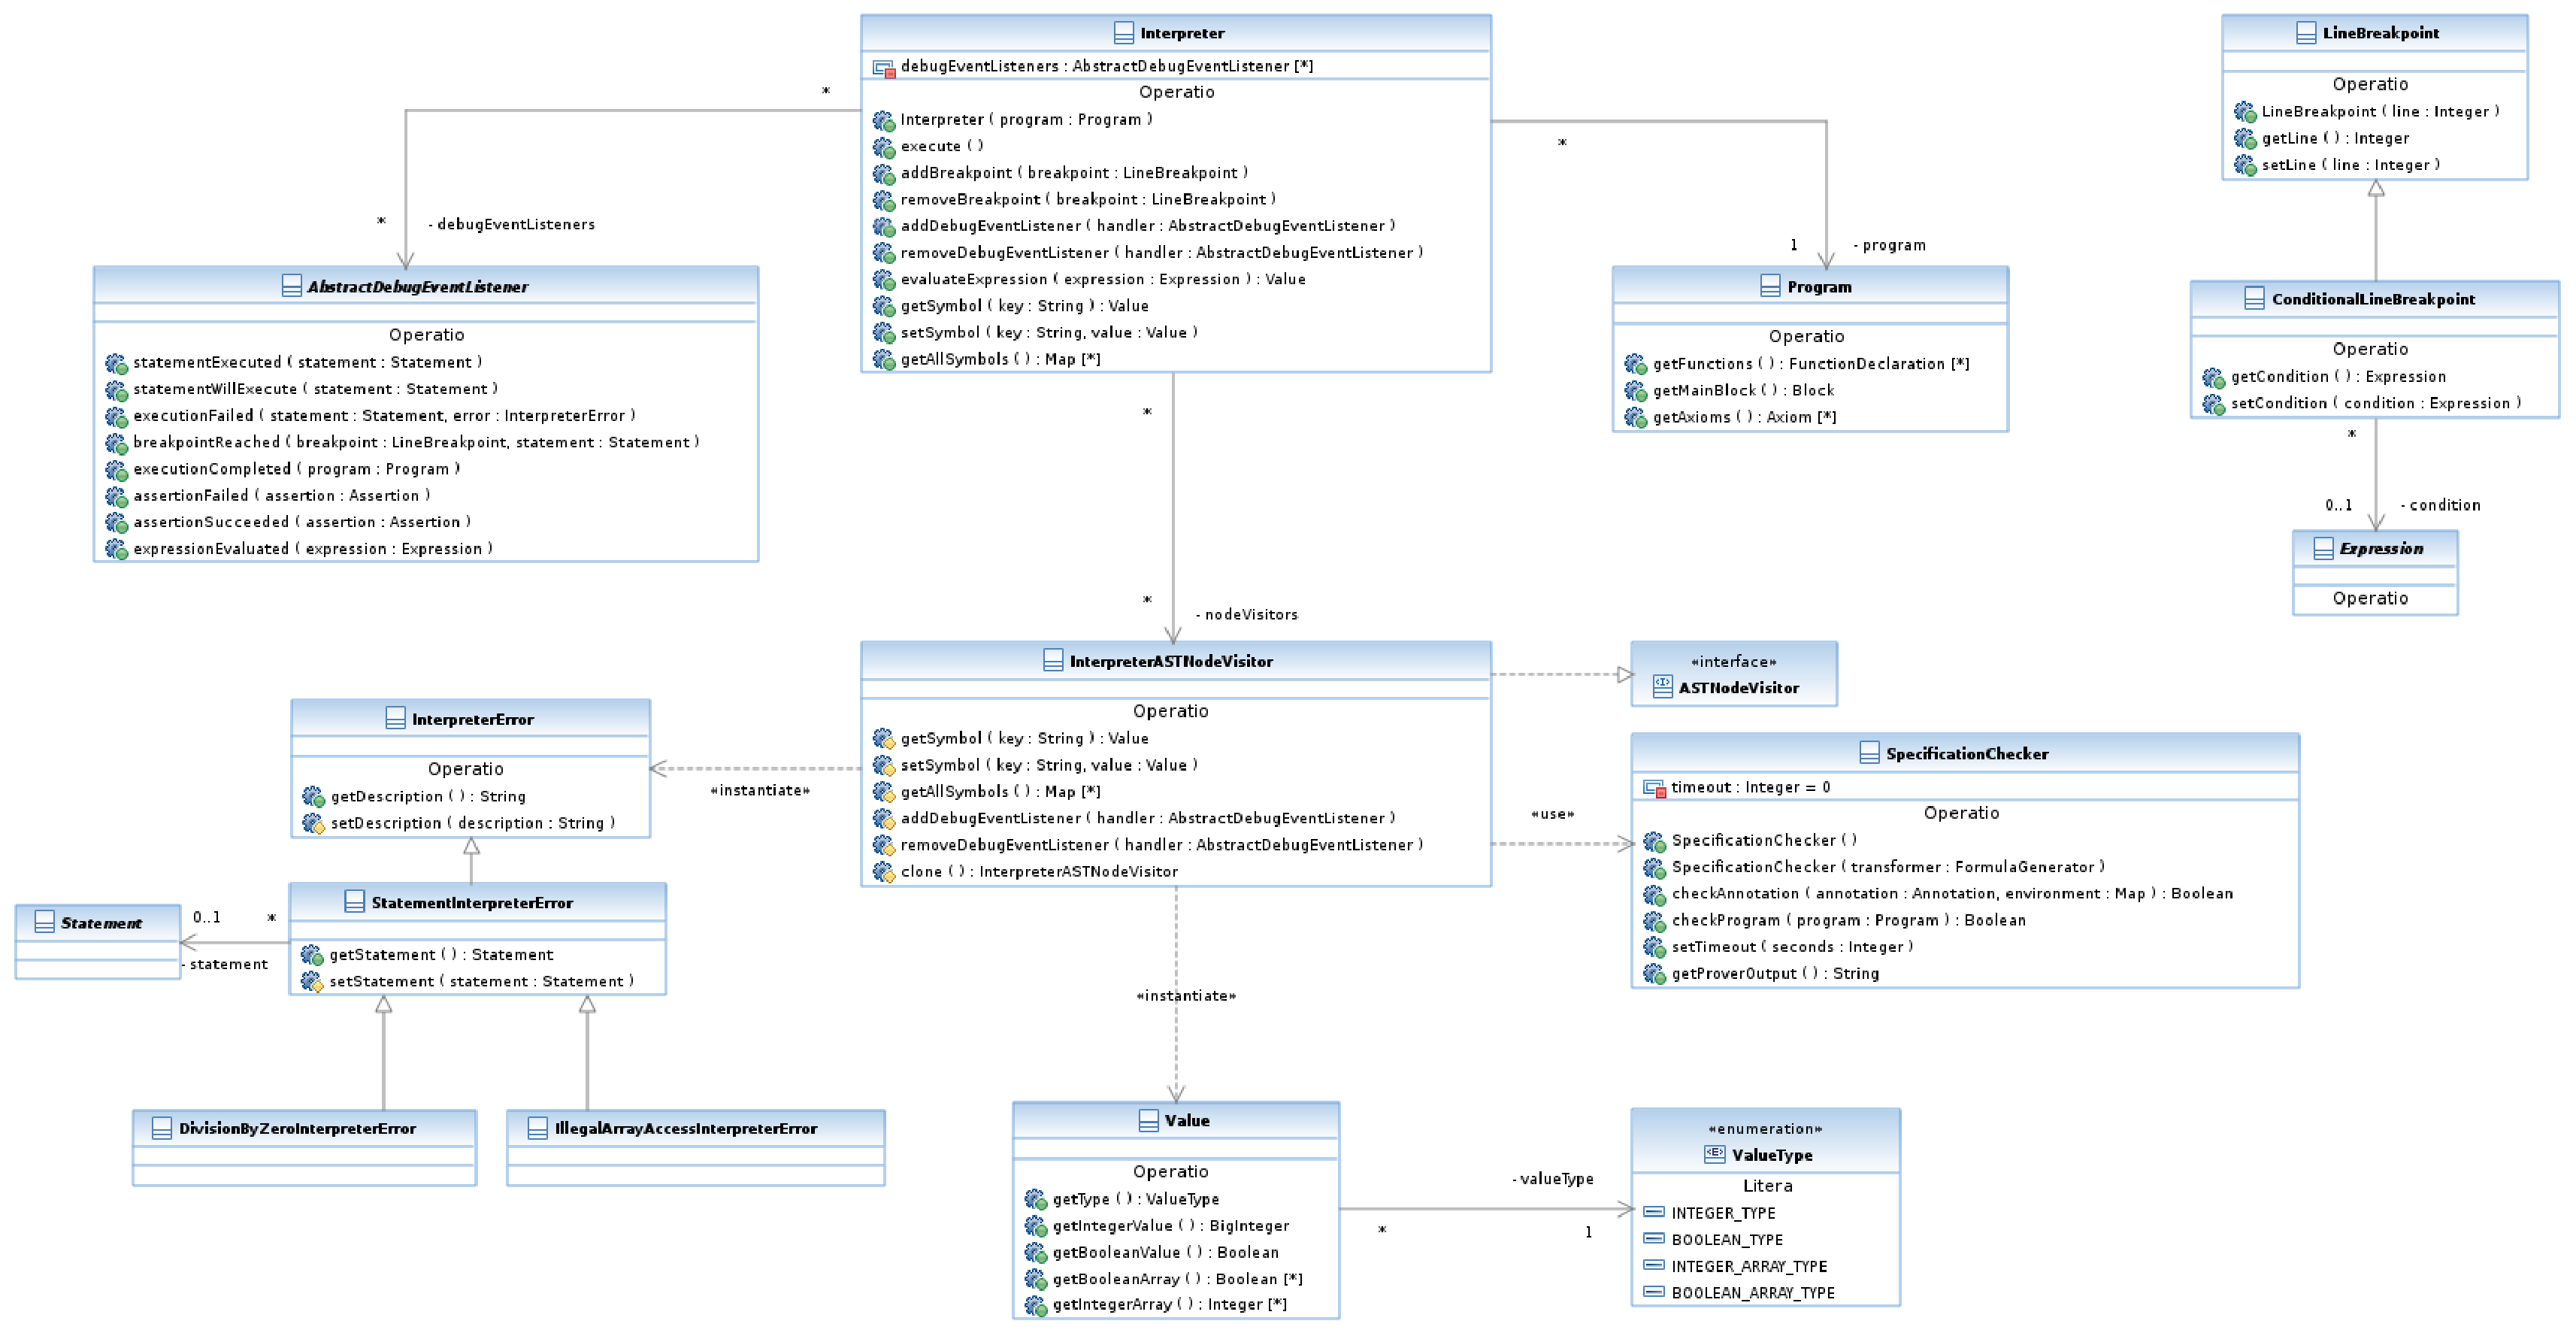
\includegraphics[angle=90,height=\textheight]{diagrams/interpreter_component.pdf}
\newpage
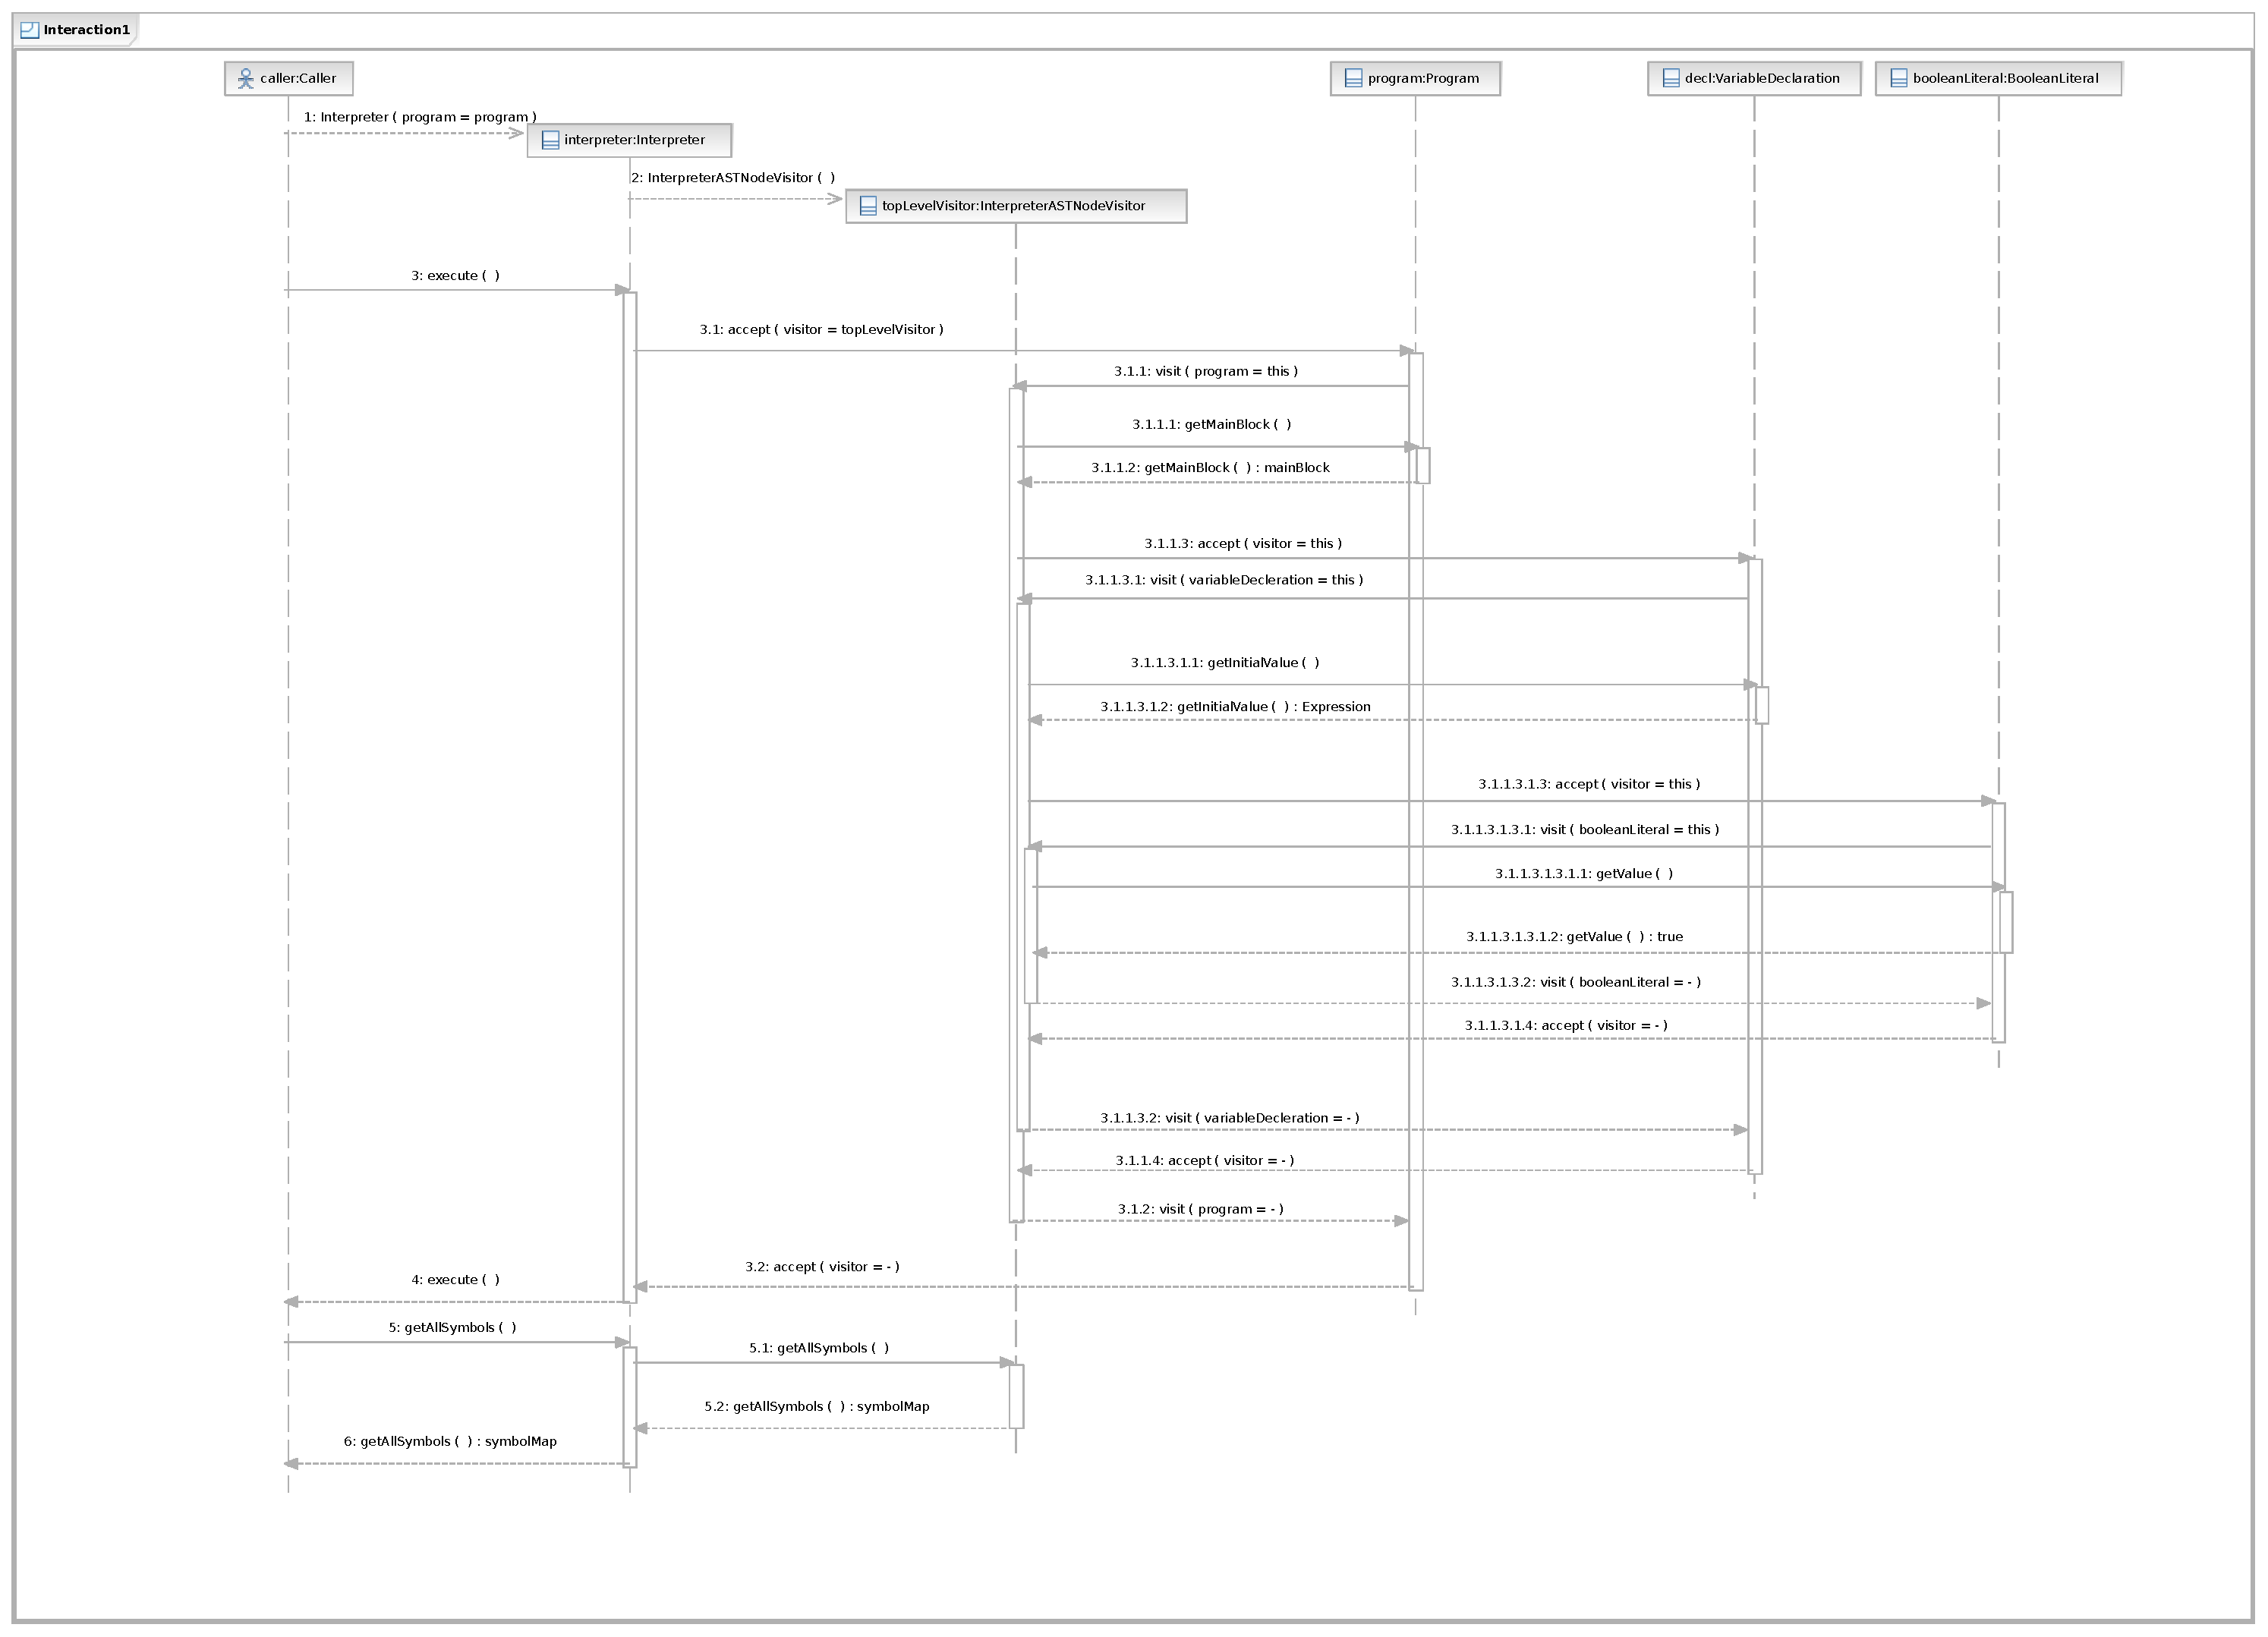
\includegraphics[angle=90,height=\textheight]{diagrams/interpreter_functioncall_sequence.pdf}
